
\textbf{Diffusion models.} 
Denoising Diffusion Implicit Models (DDIM) generate images by reversing a diffusion process~\cite{ho2020denoising, sohl2015deep, song2020score}. 
After training a denoiser $\epsilon_\theta^{t}$ and freezing its weights $\theta$, the denoising process can be seen as an ODE on rescaled noisy images $\bar{x}(t) = x(t) / \sqrt{\alpha(t)}$.
Given a prompt $y$ and current time step $t \in [0, 1]$, the denoising process satisfies:
\begin{equation}
    \label{eq:DDIM}
    \frac{d \bar{x}(t)}{dt} = \epsilon_\theta^{t} \bigl( \sqrt{\alpha(t)} \bar{x}(t), y\bigr) \frac{d \sigma(t)}{dt} \text{,}
\end{equation}
where $\bar x(1)$ is sampled from a Gaussian distribution, $\sigma(t) = \sqrt{1 - \alpha(t)}/\sqrt{\alpha(t)}$, and $\alpha(t)$ are scaling factors.
When discretized with forward Euler, this equation yields the following update to transition from step $t$ to a less noisy step $t - \tau < t$:
\begin{equation}
    \label{eq:DDIM_disc}
    \bar{x}(t - \tau) = 
    \bar{x}(t) + \epsilon_\theta^{t} \bigl( \sqrt{\alpha(t)} \bar{x}(t), y\bigr) 
    \left[ \sigma(t - \tau) - \sigma(t) \right] \text{.}
\end{equation}
The DDIM ODE can also be integrated in reverse direction to estimate $\bar x(t)$ for any $t\in[0, 1]$ from a clean image $x_0$.
This operation is called \textit{DDIM inversion} and is studied in multiple works~\cite{mokady2023null, miyake2023negative}.

\textbf{Classifier-free guidance.} 
Classifier-free guidance (CFG)~\cite{ho2022classifier} provides high-quality conditional samples without  gradients from auxilary models~\cite{dhariwal2021diffusion}. 
CFG modifies the noise prediction $\hat{\epsilon}_\theta^t$ (score function) 
by linearly combining conditional and unconditional predictions:
\begin{equation}
\epsilon_\theta^{t} \bigl( x(t), y\bigr) = 
 \hat{\epsilon}_\theta^{t} ( x(t), \varnothing ) + 
 \gamma \cdot \bigl(
\hat{\epsilon}_\theta^{t} ( x(t), y) - \hat{\epsilon}_\theta^{t} ( x(t), \varnothing )  
\bigr),
\end{equation}
where the guidance scale $\gamma$ is a scalar, with $\gamma = 0$ corresponding to unconditional sampling and $\gamma = 1$ to conditional. 
In practice, larger values $\gamma > 1$ are necessary to obtain high-quality samples at a cost of reduced diversity and extreme over-saturation.
We demonstrate the effect of different CFG values in \cref{fig:cfg_effect}. 
For the rest of the paper we use the modified CFG version of the denoiser $\epsilon_\theta^{t} \bigl( x(t), y\bigr)$.

\begin{figure}
    \centering
    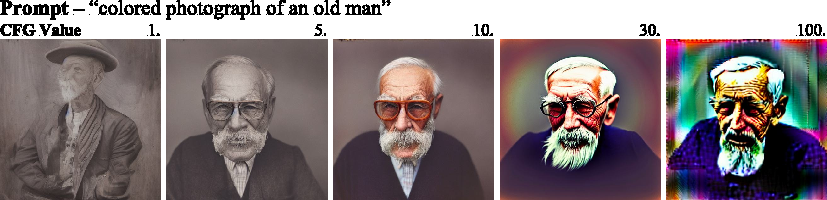
\includegraphics[width=\linewidth]{figs/cfg_effect.pdf}
    \vspace{-.25in}
    \caption{The effect of CFG values on 2D generation  with StableDiffusion 2.1 \cite{Rombach_2022_CVPR}. For small values, the model tends to ignore certain words in the prompt. For high values, images become over-saturated.}
    \label{fig:cfg_effect}
    \vspace{-.2in}
\end{figure}


\textbf{Score Distillation.} 
%
Diffusion models efficiently generate images and can learn to represent common objects from arbitrary angles~\cite{armandpour2023re} and with varying lighting~\cite{poole2022dreamfusion}.
Capitalizing on this success, Score Distillation Sampling (SDS)~\cite{poole2022dreamfusion} distills a pre-trained diffusion model $\epsilon_\theta^{t}$ to produce a 3D asset.
%
In practice, the 3D shape is usually parameterized by a NeRF~\cite{mildenhall2020nerf}, InstantNGP~\cite{muller2022instant}, or Gaussian Splatting~\cite{kerbl20233d}.
Multiple works additionally extract an explicit representation for further optimization~\cite{lin2023magic3d, tang2023make, wang2024prolificdreamer, chen2024it3d}.
We use InstantNGP~\cite{muller2022instant} to balance between speed and ease of optimization.

Denote the parameters of a differentiable 3D shape representation by $\psi \in \mathbb{R}^d$ and differentiable rendering by a function $g(\psi, c): \mathbb{R}^d \times C \rightarrow \mathbb{R}^{N\times N}$ that returns an image given camera parameters $c \in C$. 
Intuitively, in each iteration, SDS samples~$c$, renders the corresponding (image) view $g(\psi, c)$, perturbs it with $\epsilon \sim \mathcal{N}(0, I)$ to level $t \sim [0, 1]$, and denoises it with $\epsilon_\theta^{t}$; the difference between the true and predicted noise is propagated to the parameters of the 3D shape. 
More formally, after sampling the camera view $c$ and randomly drawing a time $t$, SDS renders the volume and adds Gaussian noise $\epsilon$ to obtain a noisy image $x(t) = \sqrt{\alpha(t)} g(\psi, c) + \sqrt{1 - \alpha(t)}\epsilon.$ 
Then, SDS improves the generated volume by using a gradient(-like) direction to update its parameters $\psi$:
\begin{equation}
    \label{eq:dreamfusion}
        \nabla_\psi\mathcal{L}_{SDS} = \mathbb{E}_{t, \epsilon, c}  \sigma(t) \left[\epsilon_\theta^{t}\bigl(x(t), y\bigr)  - \epsilon \right] \frac{\partial g}{\partial \psi} \text{.}
\end{equation}
We refer to the term $ \left[ \epsilon_\theta^{t}\bigl(x(t), y\bigr)  - \epsilon \right]$ as \textit{guidance} in score distillation, as it `guides' the views of the shape. In theory, this expression may not correspond to the true gradient of a function and there are many hypotheses about its effectiveness~\cite{poole2022dreamfusion, wang2023steindreamer, katzir2023noise, yu2023text, roeder2017sticking}. 
In this work, we show that instead it can be seen as a high-variance version of DDIM after a change of variables.
